% ----------------------------------------------------------
\chapter{Algoritmos e estruturas de dados para consulta de pontos no plano}\label{cap:desenvolvimento}
% ----------------------------------------------------------
Nesta seção veremos formas de construir estruturas de dados para um conjunto de pontos no plano. Consideramos que os pontos são fixos. Para cada estrutura construída, veremos também como utilizá-la para consultar pontos dentro de uma janela.

% ----------------------------------------------------------
\section{Árvore KD}
% ----------------------------------------------------------

Uma árvore KD é uma árvore binária onde cada folha é um ponto \textit{k-dimensional}.
Cada nó não-folha guarda um valor $v$ em uma dimensão $d$. Pontos cujo os valores na dimensão $d$ são iguais ou menores a $v$ estão na subárvore à esquerda, e respectivamente, pontos com valores na dimensão $d$ maiores que $v$ estão na subárvore à direita. Cada nível da árvore é associado a uma das \textit{k dimensões}. Então, a citar um exemplo no plano,
se dado nível considera o eixo $x$, a subárvore à esquerda contém os pontos com o eixo $x$ menor que o valor $v$. Similarmente, à direita contém os pontos com o eixo $x$ maior que o valor $v$. Neste caso do plano, o eixo $y$ é considerado no próximo nível da árvore.

\subsection{Árvore 2D}
Uma árvore 2D é a versão com duas dimensões para árvores KD. A sua construção considera um dado conjunto de pontos no plano ($P$) e pode ser feita da seguinte forma. Na construção de uma árvore para 2 dimensões, cada ponto tem uma forma $p = (p_x, p_y)$. Escolhemos um eixo para iniciar a construção da árvore. Ao iniciar a construção, realizamos uma $x$-ordenação e uma $y$-ordenação nos pontos de $P$ (no caso $n$ dimensional, faremos $n$ ordenações, uma para cada dimensão). Chamaremos o conjunto de pontos ordenados pelo eixo $x$ de $P_{ord(x)}$, e ordenados por $y$ de $P_{ord(y)}$.

A seguir, apresentamos uma forma de construir uma árvore 2D como em \cite{cg08}.
Fixado um eixo, o valor da mediana dos pontos ordenados neste eixo será o valor $v$ escolhido para dividir $P$ em dois subconjuntos, e serão criados dois subconjuntos. Chamamos recursivamente a construção das subárvores à esquerda e à direita de $v$ alternando o eixo e passando os subconjuntos. A base do algoritmo ocorre quando o conjunto de pontos possui um único ponto. Neste caso, armazenamos este ponto na folha da árvore.  Vamos ilustrar uma construção de uma árvore 2D considerando o conjunto de pontos da Figura \ref{fig:1}.
\begin{figure}[h!]
    \centering
    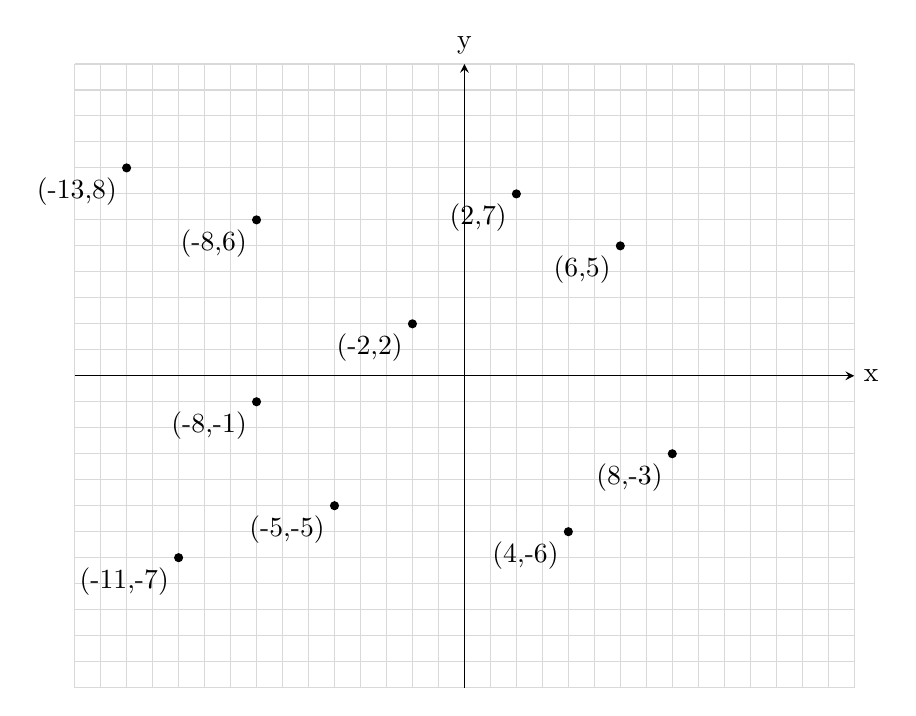
\begin{tikzpicture}[scale=0.33]
  \draw[gray!30] (-15,-12) grid[xstep=1, ystep=1]  (15,12);
  \draw[-stealth] (-15,0)--(15,0) node[right]{x}; % x axis
  \draw[-stealth] (0,-12)--(0,12) node[above]{y}; % y axis


  \fill (-13,8)  circle[radius=5pt] node[anchor=north east]{(-13,8)};
  \fill (-8,6)  circle[radius=5pt] node[anchor=north east]{(-8,6)};
  \fill (-2,2)  circle[radius=5pt] node[anchor=north east]{(-2,2)};
  \fill (-8,-1)  circle[radius=5pt] node[anchor=north east]{(-8,-1)};
  \fill (-11, -7)  circle[radius=5pt] node[anchor=north east]{(-11,-7)};
  \fill (-5,-5)  circle[radius=5pt] node[anchor=north east]{(-5,-5)};
  \fill (2,7)  circle[radius=5pt] node[anchor=north east]{(2,7)};
  \fill (6,5)  circle[radius=5pt] node[anchor=north east]{(6,5)};
  \fill (8,-3)  circle[radius=5pt] node[anchor=north east]{(8,-3)};
  \fill (4,-6)  circle[radius=5pt] node[anchor=north east]{(4,-6)};
\end{tikzpicture}
    \caption{Plano com os pontos $P$}
    \label{fig:1}
\end{figure}

Inicialmente escolhemos o eixo $x$. Acompanharemos a troca de eixos de acordo com o nível da árvore. Caso o nível seja \emph{par}, consideramos o eixo $x$, do contrário, o eixo $y$.
Realizamos uma $x$-ordenação em $P$ obtendo $P_{ord(x)} = ((-13,8), (-11,-7), (-8,6), (-8,-1),$ $(-5,5), (-2, 2), (2,7),$ $ (4,-6),(6,5),(8,-3))$. Com isso, sabemos que a $x$-mediana é $v = -5$ (veja a Figura \ref{fig:2}). Criamos dois subconjuntos $P_1$ e $P_2$ tal que: $P_1 = \{p \in P : p_x \leq v\}$ e $P_2 = \{p \in P : p_x > v\}$; e, de forma recursiva, obtemos as árvores 2D dos dois novos subconjuntos $P_1$ e $P_2$ (as raízes dessas novas árvores consideram o eixo $y$). Por fim, criamos um nó $r$ e armazenamos nele a $x$-mediana (ou seja, $v=-5)$; a subárvore à esquerda de $r$ será uma árvore 2D sobre $P_1$; e a subárvore à direita de $r$ será uma árvore 2D sobre $P_2$. % Dividimos o conjunto de pontos em dois subconjuntos: $P_1$ com os pontos com $x \leq -5$ e $P_2$ com os pontos $x > -5$. Ilustramos tais subconjuntos na Figura \ref{fig:2}  Criamos dois nós: $v_{esq}$ e $v_{dir}$, e associamos os conjuntos $P_1$ e $P_2$ nas chamadas recursivas.

%A região do nó raiz é calculada como: 
%$ -13 \leq x \leq 8 $ e $ -7 \leq y \leq 8$. 

\begin{figure}[h!]
 \centering
  \begin{tikzpicture}[x=0.25cm,y=0.25cm]
%   \draw[gray!30] (-15,-12) grid[xstep=1, ystep=1]  (15,12);
  \draw[-stealth] (-15,0)--(15,0) node[right]{x}; % x axis
  \draw[-stealth] (0,-12)--(0,12) node[above]{y}; % y axis

\draw[red] (-5,12)--(-5,-12); % y axis

  \fill (-13,8)  circle[radius=2pt] ;
  \fill (-8,6)  circle[radius=2pt] ;
  \fill (-2,2)  circle[radius=2pt] ;
  \fill (-8,-1)  circle[radius=2pt];
  \fill (-11, -7)  circle[radius=2pt];
  \fill (-5,-5)  circle[radius=2pt] node[anchor=north east]{(-5)};
  \fill (2,7)  circle[radius=2pt] ;
  \fill (6,5)  circle[radius=2pt] ;
  \fill (8,-3)  circle[radius=2pt];
  \fill (4,-6)  circle[radius=2pt];
\end{tikzpicture}
  \caption{A linha vermelha é o corte no eixo $x$}
  \label{fig:2}
\end{figure}

Vale reforçar que o eixo $y$ será considerado para os subconjuntos $P_1$ e $P_2$. Para $P_1$, realizamos uma $y$-ordenação dos pontos e obtemos $P_{1ord(y)} = ((-11,-7), (-5,-5), (-8,-1),$ $(-8,6), (-13,8))$. A $y$-mediana é $v=-1$. O processo continua com a criação dos subconjuntos considerando $P_1$ e depois considerando os pontos em $P_2$. A Figura \ref{fig:3} mostra os cortes no plano utilizados para construir os subconjuntos de pontos. %Criamos um nó e armazenamos nele o valor $v=-1$. Note que com isso, o conjunto de pontos é mais uma vez dividido em $((-11,7), (-5,-5), (-8,-1))$ e $((-8,6), (-13,8))$.

%Sabemos que o eixo foi cortado em $-5$ em $x$.
%Calculamos a região do $nó_{-1}$ que conterá os pontos $(x,y)$ tal que: $-11 \leq x < -5 \textmd{; e } -5 \leq y < 8$.
 
\begin{figure}[h!]
    \centering
    \begin{tikzpicture}[x=0.25cm,y=0.25cm]
%   \draw[gray!30] (-15,-12) grid[xstep=1, ystep=1]  (15,12);
  \draw[-stealth] (-15,0)--(15,0) node[right]{x}; % x axis
  \draw[-stealth] (0,-12)--(0,12) node[above]{y}; % y axis
  \draw[red] (-5,12)--(-5,-12); % y axis
  \draw[green] (-15,-1)--(-5,-1); % y axis
  \fill (-13,8)  circle[radius=2pt] ;
  \fill (-8,6)  circle[radius=2pt] ;
  \fill (-2,2)  circle[radius=2pt] ;
  \fill (-8,-1)  circle[radius=2pt] node[anchor=north east]{(-1)};
  \fill (-11, -7)  circle[radius=2pt];
  \fill (-5,-5)  circle[radius=2pt] ;
  \fill (2,7)  circle[radius=2pt] ;
  \fill (6,5)  circle[radius=2pt] ;
  \fill (8,-3)  circle[radius=2pt];
  \fill (4,-6)  circle[radius=2pt];
\end{tikzpicture}
    \caption{A linha verde é o corte no eixo $y$ que divide em relação ao ponto $(-8, -1)$ }
    \label{fig:3}
\end{figure}


Este procedimento é repetido até que o conjunto de pontos tenha somente um ponto. Neste caso, criamos um nó folha, contendo o ponto $p$. As Figuras \ref{fig:4} e \ref{fig:5} Ilustra todos os cortes sobre o conjunto de pontos inicial. Estes cortes foram utilizados na construção dos subconjuntos de pontos. % e utilizados para  e a construção da árvore 2D correspondente.% sentação dos pontos no plano com os eixos de corte para a construção da árvore 2D.

\begin{figure}[h!]
    \centering
   \begin{tikzpicture}[x=0.25cm,y=0.25cm]
%   \draw[gray!30] (-15,-12) grid[xstep=1, ystep=1]  (15,12);
  \draw[-stealth] (-15,0)--(15,0) node[right]{x}; % x axis
  \draw[-stealth] (0,-12)--(0,12) node[above]{y}; % y axis
  \draw[gray] (-5,12)--(-5,-12); % y axis
  \draw[gray] (-15,-1)--(-5,-1); % y axis
  \draw[gray] (15,2)--(-5,2); % y axis
  \draw[gray] (-8,-1)--(-8,-12); % y axis
  \draw[gray] (-13,-1)--(-13,12); % y axis
  \draw[gray] (4,2)--(4,-12); % y axis
  \draw[gray] (2,2)--(2,12); % y axis
  
  \draw[gray] (-15,-7)--(-8,-7); % y axis
  \draw[gray] (4,-6)--(15,-6); % y axis
  
  \fill (-13,8)  circle[radius=2pt]node[anchor=north east]{(-13)};
  \fill (-8,6)  circle[radius=2pt] ;
  \fill (-2,2)  circle[radius=2pt] node[anchor=north east]{(2)};
  \fill (-8,-1)  circle[radius=2pt] node[anchor=north east]{(-8)};
  \fill (-11, -7)  circle[radius=2pt];
  \fill (-5,-5)  circle[radius=2pt] node[anchor=north east]{(-5)} ;
  \fill (2,7)  circle[radius=2pt] ;
  \fill (6,5)  circle[radius=2pt] ;
  \fill (8,-3)  circle[radius=2pt];
  \fill (4,-6)  circle[radius=2pt] node[anchor=north east]{(4)};
\end{tikzpicture}
    \caption{Plano $P$ com a subdivisão dos pontos e as linhas cinza são os cortes dos nós da árvore 2D}
    \label{fig:4}
\end{figure}

% A árvore 2D correspondente à figura anterior e o pseudocódigo
%para a construção de uma árvore 2D são dados em seguida.
A Figura \ref{fig:5} ilustra a árvore 2D completa para o conjunto de pontos considerados anteriormente. Logo depois, descrevemos um algoritmo que constrói uma árvore 2D para um dado conjunto de pontos no plano. 

\begin{figure}
    \centering
    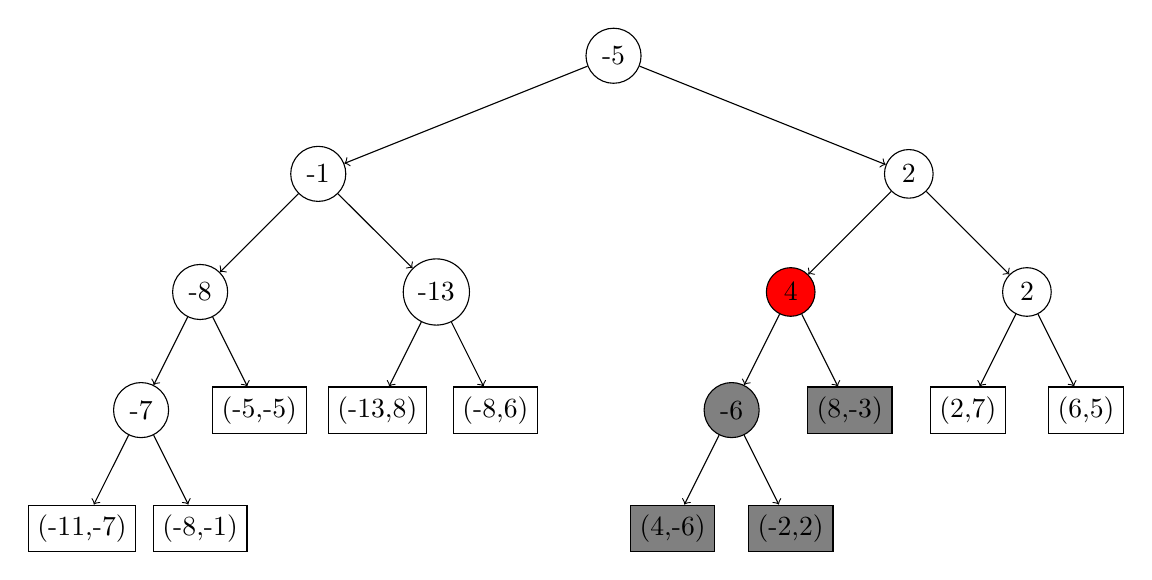
\begin{tikzpicture}[nodes={draw, circle}, ->]
    % Tree structure
 \node{-5}
    child { node {-1} 
        child { node {-8}
            child{ node{-7}
                child{ node[rectangle]{(-11,-7)}}
                child{ node[rectangle]{(-8,-1)}}
            }
            child { node[rectangle]{(-5,-5)}}
        }
        child [missing]
        child { node {-13}
            child { node[rectangle]{(-13,8)}}
            child { node[rectangle]{(-8,6)}}
        }
    }
    child [missing]
    child [missing]
    child [missing]
    child [missing]
    child { node {2} 
        child { node[fill=red]{4}
            child{node[fill=gray]{-6}
                child {node[rectangle, fill=gray]{(4,-6)}  }
                child {node[rectangle ,fill=gray]{(-2,2)}  }
            }
            child{node[rectangle, fill=gray]{(8,-3)}}
        }
        child [missing]
        child { node{2}
            child{node[rectangle]{(2,7)}}
            child{node[rectangle]{(6,5)}}
        }
    };
\end{tikzpicture}
    \caption{Árvore 2D construída. O $nó_{4}$ indica a área da Figura 6}
    \label{fig:5}
\end{figure}

\begin{algorithm}[h!]
    \caption{Recebe um conjunto de pontos $P$ no plano e uma profundidade da árvore. Devolve a raiz de uma árvore 2D.}
    \begin{algorithmic}[1]
        \Function{ConstróiÁrvore2D}{$P$, $profundidade$}
            \If{$P$ contém apenas um ponto}
                \Return nó folha que armazena o ponto de $P$
            \Else
                \If{$profundidade$ é par}
                    \State Faça uma $x$-ordenação sobre $P$
                    \State Divide $P$ em dois subconjuntos pela $x$-mediana ($v$) 
                    \State Seja $P_1$ o conjunto dos pontos à esquerda de $v$
                    \State Seja $P_2$ o conjunto de pontos à direita de $v$
                \Else
                    \State Faça uma $y$-ordenação sobre $P$
                    \State Divide $P$ em dois subconjuntos pela $y$-mediana ($v$)
                    \State Seja $P_1$ o conjunto dos pontos abaixo de $v$
                    \State Seja $P_2$ o conjunto de pontos acima de $v$
                \EndIf
            \EndIf
            \State Cria os nós $r_{esquerda}$ e $r_{direita}$
            \State $v_{esquerda} \leftarrow $ \Call{ConstróiÁrvore2D}{$P_1, profundidade+1$}
            \State $v_{direita} \leftarrow $ \Call{ConstróiÁrvore2D}{$P_2, profundidade+1$}
            \State Cria um nó $r$, armazene em $r$ o valor $v$ e associe os filhos $r_{esquerda}$ e $r_{direita}$ 
            \State \Return $r$
        \EndFunction
    \end{algorithmic}
\end{algorithm}

\subsection{Consulta de pontos em árvores 2D}

Uma consulta em uma árvore 2D construída sobre um conjunto de pontos $P$ é uma busca de quais pontos de $P$ estão entre um retângulo de consulta
\([x,x']  \times  [y,y']\) que chamaremos de janela. Um ponto $p = (p_x, p_y)$ está dentro de um retângulo de busca se $p_x \in [x, x'] \textrm{ e } p_y \in [y, y']$. Podemos dizer que uma consulta no plano é composta de duas subconsultas nos eixos: uma no eixo $x$ e outra no eixo $y$.

%Denotaremos uma região de um nó \(r\) como \(região(r)\). Portanto, o algoritmo de consulta buscará pela subárvore com raiz \(r\) somente se o retângulo de busca intersectar a \(região(r)\).

Seja $P^r$ o conjunto de pontos em folhas alcançáveis a partir de $r$. Podemos definir uma \emph{região} retangular a partir dos pontos em $P^r$ (denotamos tal região por região($r$)): %Então, a $região(r)$, que é um retângulo no plano, pode ser definida através do intervalo:
$$
 \mbox{região}(r) = \begin{cases} \min_x(p) \leq x \leq \max_x(p),\ \forall p \in P^r\\ \min_y(p) \leq y \leq \max_y(p),\ \forall p \in P^r \end{cases} 
$$

O algoritmo de consulta buscará pela subárvore com raiz \(r\) somente se o retângulo de busca intersectar a região($r$). Um exemplo de uma região de um nó de uma árvore 2D pode ser observado na Figura \ref{fig:5}. A região do nó$_4$ (que guarda o valor 4) é
$$
\mbox{região}(\mbox{nó}_4) =  \begin{cases} -2 \leq x \leq 8 \\ -6 \leq y \leq 2 \end{cases} 
$$

Dada uma janela de consulta, o algoritmo de busca funciona descendo a árvore, mas visitando somente os nós $r$ cuja
\(\mbox{região}(r)\) intersecta a janela. Quando uma \(\mbox{região}(r)\) está contida na janela de consulta, devolvemos todos os pontos na subárvore enraizada em $r$. No caso em que chegamos em um nó folha, temos que verificar se o nó está dentro da janela, e se estiver, devolvê-lo.

\begin{figure}[h!]
    \centering
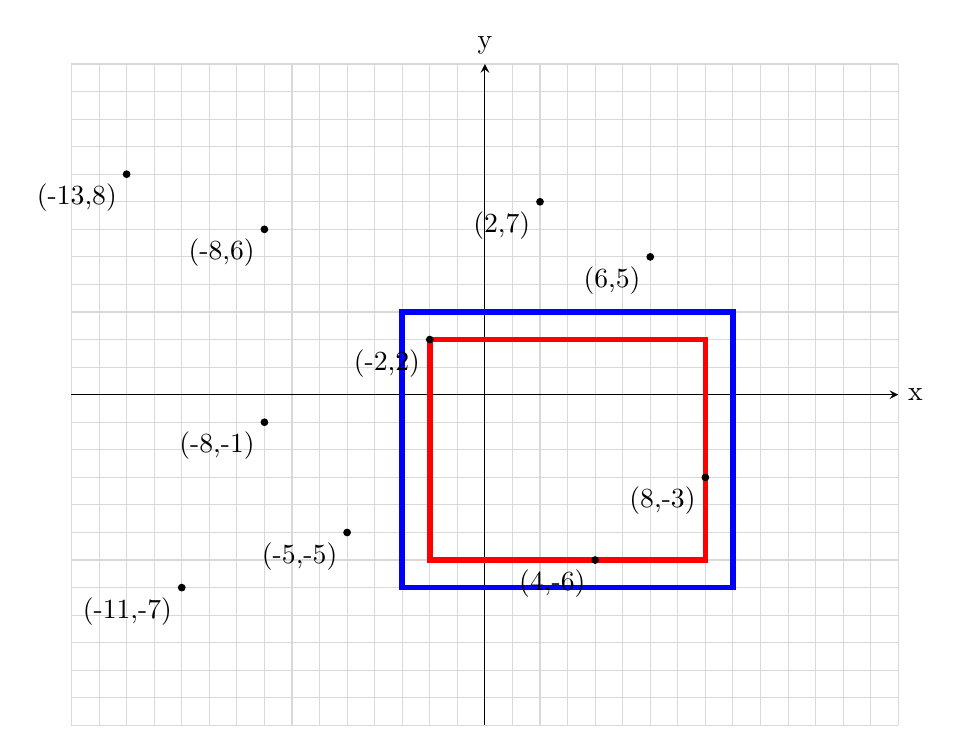
\begin{tikzpicture}[scale=0.35]
  \draw[gray!30] (-15,-12) grid[xstep=1, ystep=1]  (15,12);
  \draw[-stealth] (-15,0)--(15,0) node[right]{x}; % x axis
  \draw[-stealth] (0,-12)--(0,12) node[above]{y}; % y axis

\draw[draw=red, line width=2pt] (-2,-6) rectangle (8,2);
  \draw[draw=blue, line width=2pt] (-3,-7) rectangle (9,3);

  \fill (-13,8)  circle[radius=4pt] node[anchor=north east]{(-13,8)};
  \fill (-8,6)  circle[radius=4pt] node[anchor=north east]{(-8,6)};
  \fill (-2,2)  circle[radius=4pt] node[anchor=north east]{(-2,2)};
  \fill (-8,-1)  circle[radius=4pt] node[anchor=north east]{(-8,-1)};
  \fill (-11, -7)  circle[radius=4pt] node[anchor=north east]{(-11,-7)};
  \fill (-5,-5)  circle[radius=4pt] node[anchor=north east]{(-5,-5)};
  \fill (2,7)  circle[radius=4pt] node[anchor=north east]{(2,7)};
  \fill (6,5)  circle[radius=4pt] node[anchor=north east]{(6,5)};
  \fill (8,-3)  circle[radius=4pt] node[anchor=north east]{(8,-3)};
  \fill (4,-6)  circle[radius=4pt] node[anchor=north east]{(4,-6)};
  

\end{tikzpicture}
\caption{Em vermelho a região do nó da árvore anterior com o valor 4 armazenado}
\label{fig:6}
\end{figure}

Segue o algoritmo que recebe como parâmetros a raiz de uma árvore 2D e uma janela $R$.
Usamos uma chamada \Call{ReportaSubárvore}{$r$} que atravessa a árvore do nó \(r\) e devolve todos os pontos nas suas folhas. Segue como notação \(filho_{esq}(r)\) sendo o filho à esquerda e \(filho_{dir}(r)\) o filho à direita do nó \(r\).


\begin{algorithm}[H]
    \caption{Recebe como parâmetro um nó $r$ e uma janela $R$. Devolve todos os pontos dentro de $R$.}
    \begin{algorithmic}[1]
    \Function{ConsultaEmÁrvore2D}{$r$, $R$}
        \If{v é folha}
        \Return  $v$ se estiver dentro da $R$
        \Else
            \If{$\mbox{região}(filho_{esq}(r))$ está contido na $R$}
            \State \Return \Call{ReportaSubárvore}{$filho_{esq}(r)$}
            \Else
                \If{$\mbox{região}(filho_{esq}(r))$ intersecta $R$}
                \State \Return \Call{ConsultaEmÁrvore2D}{$filho_{esq}(r)$, $R$}
                \EndIf
            \EndIf
            \If{$\mbox{região}(filho_{dir}(r))$ está contido na $R$}
                \State \Return \Call{ReportaSubávore}{$filho_{dir}(r)$, $R$}
            \Else
                \If{$\mbox{região}(filho_{dir}(r))$ intersecta $R$}
                \State \Return \Call{ConsultaEmÁrvore2D}{$filho_{dir}(r)$, $R$}
                \EndIf
            \EndIf
        \EndIf
    \EndFunction
    \end{algorithmic}
\end{algorithm}

Vamos acompanhar uma consulta na árvore construída da Figura \ref{fig:5}. Considere uma janela $[-3, 9]\times[-7, 3]$. %consulta $ -3 \leq x \leq 9 $ e $-7 \leq y < 3$. 
Iniciamos no nó$_-5$. Como o nó não é folha, checamos se a região do filho à esquerda esta dentro da consulta. O $\mbox{nó}_{-1}$ tem região $ -13 \leq x \leq -5 $ e  $ -7 \leq y \leq 8$, logo a região não está contida na consulta. Assim como a região do nó$_2$. Porém, as regiões dos $\mbox{nó}_2$ e $\mbox{nó}_{-1}$ intersectam o retângulo da consulta. Então procedemos com a consulta em ambos os nós. %chamando \Call{BuscaEmArvore}{$\mbox{nó}_{-1}$, consulta} e \Call{BuscaEmArvore}{$\mbox{nó}_{2}$, consulta}. 
Note que o filho à esquerda do $\mbox{nó}_{2}$ ($\mbox{nó}_4$ em destaque na Figura \ref{fig:5}) possui região contida na janela de consulta. Portanto todos os pontos das folha alcançáveis a partir deste nó estão na janela. 

\subsection{Otimização para a construção de uma árvore 2D}
A forma como implementamos o algoritmo de construção realiza ordenações em cada chamada.
Uma otimização para a implementação da construção da árvore 2D considera apenas 2 ordenações, uma para cada eixo. %, onde $d$ é o número de dimensões da árvore KD.
Para isto, é preciso ordenar os pontos nos dois eixos antes do inicio da construção da árvore e, a cada chamada do algoritmo que constrói a árvore, conseguimos construir os subconjuntos de pontos ordenados em tempo linear, sempre considerando uma ordenação do conjunto de pontos que originou essa chamada. % e durante a troca de eixo da árvore, é checar quais pontos no nó pai foram removidos e desconsiderá-los no eixo atual.
Por último, a Figura \ref{fig:7} corresponde a uma figura gerada por nossa implementação da árvore 2D. Como esperado, os pontos dentro de uma janela foram encontrados.
\begin{figure}[ht!]
    \begin{center}
        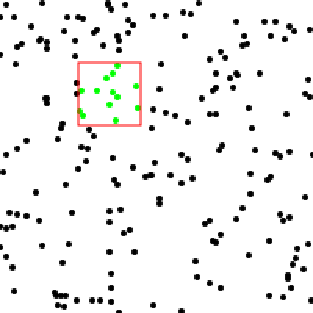
\includegraphics{images/points.pdf}
    \end{center}
    \caption {Resultados de busca em uma árvore 2D}
    \label{fig:7}
\end{figure}

%\clearpage



% ----------------------------------------------------------
\section{Árvore de Alcance}
% ----------------------------------------------------------

Uma árvore de alcance pode ser implementada considerando várias dimensões. No caso geral, com $k$ dimensões, teremos $k$ níveis de árvores binárias de busca todas balanceadas. Uma dimensão está relacionada a cada nível. O primeiro nível é formado por uma árvore binária de busca balanceada relacionada a dimensão, digamos, 1. Cada nó desta árvore guarda um valor da dimensão 1, mais uma outra árvore binária de busca balanceada relacionadas à dimensão 2. Cada nó do segundo nível, guarda uma valor da dimensão 2, mais uma outra árvore relacionada à dimensão 3. E assim por diante. Neste trabalho consideramos uma árvore de alcance para 2 dimensões (2D). Denotamos por $\tau_r$ a raiz de uma árvore relacionada a um nó $r$. Neste caso, o nó $r$ em um nível e $\tau_r$ no nível seguinte \cite{dsp_rt1}. A Figura \ref{fig:8} ilustra uma árvore de alcance 2D. Note que as folhas da árvore do primeiro nível (à esquerda) aparecem como folhas em uma árvore do segundo nível (à direita). % de uma  Para o caso com  onde cada nó não folha é um ponto $k$-dimensional
%onde guarda um valor $v$ em uma dimensão $d$ e uma árvore binária auxiliar $\tau$. Para cada $k$-dimensão
%existirá uma árvore auxiliar $\tau$ para cada dimensão.\cite{dsp_rt1}

\begin{figure}[htb!]
    \begin{center}
        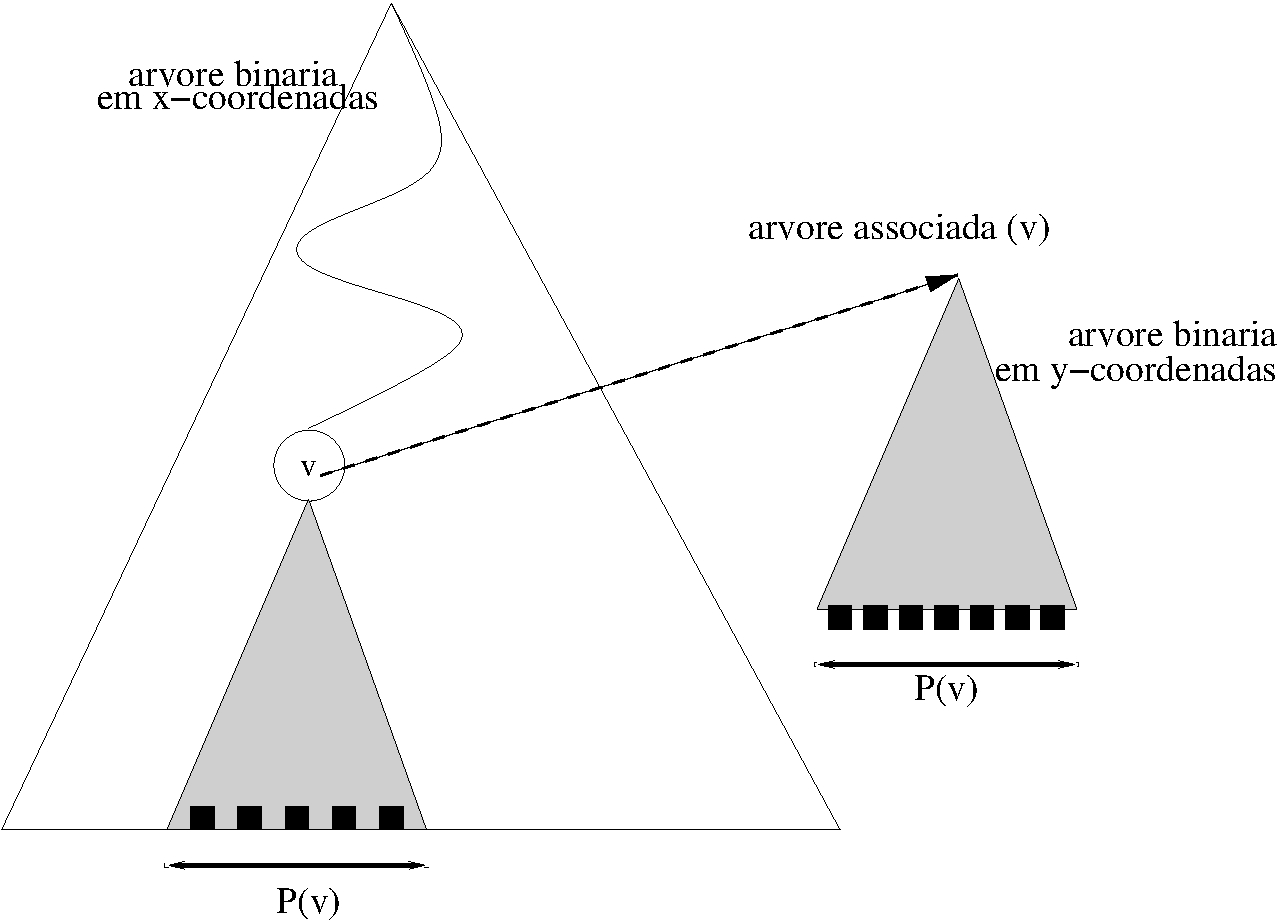
\includegraphics[scale=0.5]{images/range_tree1.pdf}
    \end{center}
    \caption{\label{fig:Fig_26} — Árvore de Alcance 2D}
    \label{fig:8}
\end{figure}

\subsection{Árvore de Alcance 2D}

Uma árvore de alcance 2D é uma versão de duas dimensões para a árvores de alcance. A construção considera um dado conjunto de pontos $P$ e pode ser feita da seguinte forma.
Temos os pontos na forma $p = (p_x, p_y)$. Ao iniciar a construção, fixamos o eixo $x$ para o primeiro nível; construímos uma árvore binária de busca balanceada $T$ considerando os valores na $x$-coordenada dos pontos de $P$; para cada nó não folha $r$ de $T$ construiremos uma árvore auxiliar $\tau_r$ com todos as folhas alcançáveis a partir de $r$. Estas árvores serão construídas considerando os valores da $y$-coordenada. Por fim, associamos $\tau_r$ ao nó $r$. Os nós folhas das árvores guardarão os pontos de $P$.

Vamos considerar o seguinte conjunto de pontos $P$ da Figura \ref{fig:9} para ilustrar a construção de uma árvore de alcance 2D.
\begin{figure}[H]
\centering
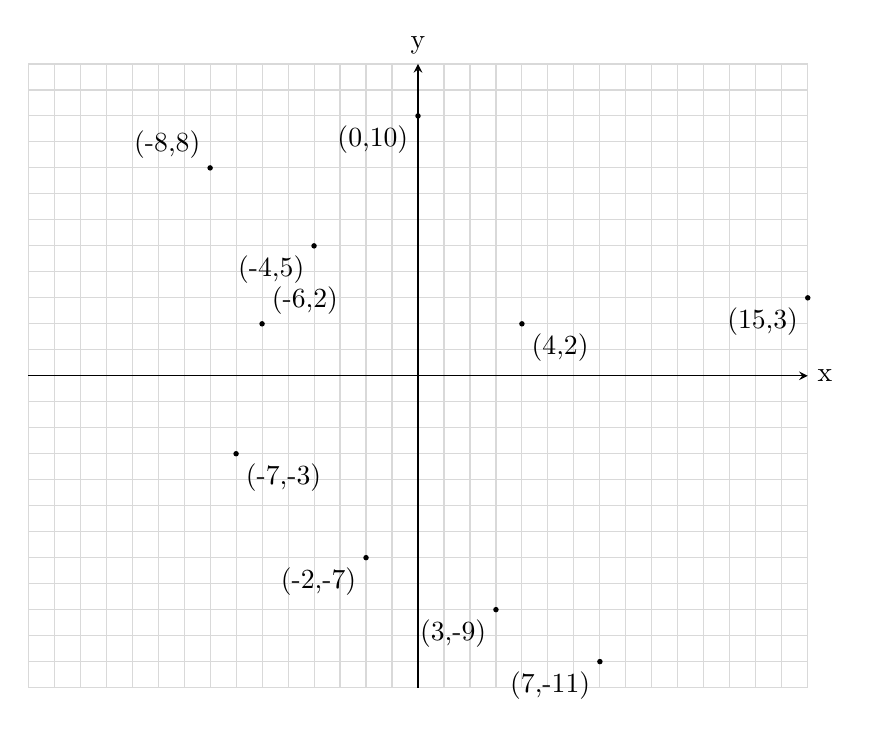
\begin{tikzpicture}[scale=0.33]
  \draw[gray!30] (-15,-12) grid[xstep=1, ystep=1]  (15,12);
  \draw[-stealth] (-15,0)--(15,0) node[right]{x}; % x axis
  \draw[-stealth] (0,-12)--(0,12) node[above]{y}; % y axis


  \fill (15,3)  circle[radius=3pt] node[anchor=north east]{(15,3)};
  \fill (-4,5)  circle[radius=3pt] node[anchor=north east]{(-4,5)};
  \fill (-6,2)  circle[radius=3pt] node[anchor=south west]{(-6,2)};
  \fill (-2,-7)  circle[radius=3pt] node[anchor=north east]{(-2,-7)};
  \fill (3,-9)  circle[radius=3pt] node[anchor=north east]{(3,-9)};
  \fill (0,10)  circle[radius=3pt] node[anchor=north east]{(0,10)};
  \fill (7,-11)  circle[radius=3pt] node[anchor=north east]{(7,-11)};
  \fill (-7,-3)  circle[radius=3pt] node[anchor=north west]{(-7,-3)};
  \fill (-8,8)  circle[radius=3pt] node[anchor=south east]{(-8,8)};
  \fill (4,2)  circle[radius=3pt] node[anchor=north west]{(4,2)};

\end{tikzpicture}
\caption{Pontos $P$ no plano}
\label{fig:9}
\end{figure}
% imagem

Para construir uma árvore binária de busca balanceada do primeiro nível, podemos inicialmente ordenar os pontos de $P$ pela %  é necessário que os pontos estejam ordenados.
%Ordenamos os pontos $P$ pela 
$x$-coordenada. %inicialmente. 
Pegamos o ponto médio da $x$-coordenada, $x_{med}$, e o guardamos em um nó $r$ da árvore. Depois, criamos dois subconjuntos $P_1$ e $P_2$ tal que $P_1 = \{p \in P : p_x \leq x_{med}\}$ e $P_2 = \{p \in P : p_x > x_{med}\}$. Criamos uma árvore binária de busca balanceada $\tau_r$ considerando o valor da $y$-coordenada dos pontos de $P$. A árvore de segundo nível associada ao vértice $r$ será $\tau_r$. O processo continua de forma recursiva sobre os dois novos conjuntos $P_1$ e $P_2$. Em seguida, adicionamos o pseudocódigo deste procedimento.

\begin{algorithm}[h!]
    \caption{Recebe como entrada um conjunto de pontos $P$. Devolve o nó raiz de uma árvore de alcance 2D.}
    \begin{algorithmic}[1]
    \Function{ConstróiÁrvoreAlcance2D}{$P$}
    \State Criamos um novo nó $r$
        \State Construímos uma árvore binária de busca balanceada associada ao nó $r$ sobre os pontos $P$ e considerando a $y$-coordenada. A árvore será denotada por $\tau_r$.%: Constrói uma árvore binária $\tau_r$ no conjunto de pontos $P_y$  de $y$-coordenadas dos pontos em $P$. Nas folhas de de $\tau_{associada}$ guardaremos os pontos em si.
        \If{$P$ contém apenas um ponto}
            \State Guardamos o ponto de $P$ em $r$.
            \State Associamos $\tau_r$ ao nó $r$. %Cria um nó $r$ guardando o ponto e fazemos $\tau_{associada}$ a árvore associada à $v$.
            
        \Else
            \State Dividimos $P$ em dois subconjuntos. 
            \State $P_1$ contém os pontos com a $x$-coordenada $\leq$ que $x_{med}$.
            \State $P_2$ contém os pontos com $x$-coordenada $>$ que $x_{med}$.
            \State $v_{esq} \leftarrow $ \Call{ConstróiÁrvoreAlcance2D}{$P_1$}.
            \State $v_{dir} \leftarrow $ \Call{ConstróiÁrvoreAlcance2D}{$P_2$}.
            \State Criamos um nó $v$ guardando $x_{med}$.
            \State Fazemos $v_{esq}$ e $v_{dir}$ filhos à esquerda e à direita de $v$.
            \State Associamos $\tau_{r}$ ao nó $r$.
        \EndIf
    \State\Return $v$
    \EndFunction
    \end{algorithmic}
\end{algorithm}

%pseudo codigo

Vamos seguir alguns passos da construção de uma árvore de alcance. Considere os os pontos da Figura \ref{fig:9} ordenados pelo eixo $x$: $P_{ord(x)} = \{(-8,8), (-7, -3), (-6, 2), (-4,5),$ $(-2,-7),(0,10), (3,-9), (4,2), (7,-11), (15,3)\}$. Criamos um nó raiz $r$ e nele armazenamos o valor da $x_{med} = -2$. Dividimos o conjunto de pontos em dois subconjuntos $P_1$ com os pontos $x\leq -2$ e $P_2$ com os valores $x > -2$.
Com relação à árvore de segundo nível relacionada ao conjunto $p$ inicial, fazemos uma $y$-ordenação nos pontos de $P$ e construímos uma árvore binária balanceada considerando os valores do eixo $y$ e associaremos a árvore resultante à raiz $r$ (ou nó$_{-2}$) da árvore do primeiro nível. A subárvore à esquerda de $r$ será uma árvore de alcance sobre $P_1$; e a subárvore à direita de $r$ será uma árvore de alcance sobre $P_2$.
A Figura \ref{fig:10} ilustra o $nó_{-6}$ e a sua árvore associada de segundo nível.
% arvore com nó 1 e nó 2, nó_2 indicando a árvore associada construida 
\begin{figure}[h!]

\centering
\begin{minipage}{.5\textwidth}
  \centering
  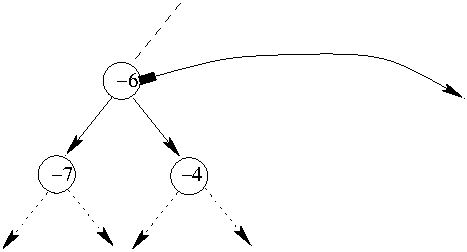
\includegraphics[width=.8\linewidth]{images/range_tree3.pdf}

  \label{fig:test1}
\end{minipage}%
\begin{minipage}{.5\textwidth}
  \centering
  \resizebox{.8\textwidth}{!}{
   \begin{tikzpicture}[nodes={draw, circle}, ->]
 \node{2}
    child { node {-3} 
        child{ node{-7}
            child{ node[rectangle]{(-2,-7)}}
            child{ node[rectangle]{(-7,-3)}}
        }
        child{ node[rectangle]{(-6,2)}}
    }
    child [missing]
    child [missing]
    child [missing]
    child [missing]
    child { node {5}
        child{ node[rectangle]{(-4,5)}}
        child{ node[rectangle]{(-8,8)}}
    };
\end{tikzpicture}
}
  
  \label{fig:test2}
 
\end{minipage}
 \caption{$nó_{-6}$ e sua $y$-árvore associada}
 \label{fig:10}
\end{figure}

Este procedimento é repetido até que o conjunto de pontos tenha somente um ponto. Neste caso, criamos um nó folha contendo o ponto $p$. A Figura \ref{fig:11} a seguir é a representação dos pontos no plano em uma árvore de alcance atingíveis do $nó_{-6}$.

\begin{figure}[h!]

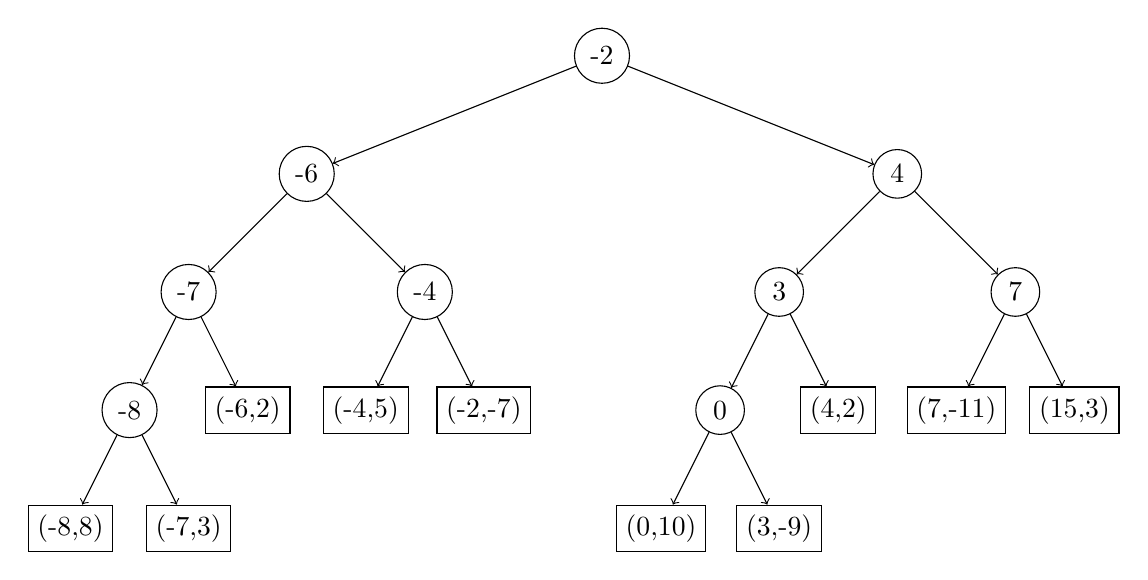
\begin{tikzpicture}[nodes={draw, circle}, ->]
    % Tree structure
 \node{-2}
    child { node {-6} 
        child { node {-7}
            child{ node{-8}
                child{ node[rectangle]{(-8,8)}}
                child{ node[rectangle]{(-7,3)}}
            }
            child { node[rectangle]{(-6,2)}}
        }
        child [missing]
        child { node {-4}
            child { node[rectangle]{(-4,5)}}
            child { node[rectangle]{(-2,-7)}}
        }
    }
    child [missing]
    child [missing]
    child [missing]
    child [missing]
    child { node {4} 
        child { node{3}
            child{node{0}
                child {node[rectangle]{(0,10)}  }
                child {node[rectangle]{(3,-9)}  }
            }
            child{node[rectangle]{(4,2)}}
        }
        child [missing]
        child { node{7}
            child{node[rectangle]{(7,-11)}}
            child{node[rectangle]{(15,3)}}
        }
    };
 \end{tikzpicture}
 \caption{Árvore construída com os pontos $P$ pela $x$-coordenada}
 \label{fig:11}
\end{figure}

\subsection{Consulta dos pontos em árvores de alcance}

Uma consulta 2-dimensional em $P$ é uma busca de quais pontos de $P$ estão entre uma janela de consulta
$[x, x'] \times [y, y']$. Um ponto $p = (p_x, p_y)$ está dentro de um retângulo de consulta se e somente
se $p_x \in [x, x']$ e $p_y \in [y, y']$. \cite{cg_rt1}

Uma consulta em uma árvore de alcance é a combinação de $n$ consultas em árvore, onde $n$ é a dimensão
da árvore de alcance.
Na árvore de alcance 2-dimensional temos uma consulta no eixo $x$ seguida por uma consulta na arvore 
auxiliar $\tau$ que foi construída considerando $y$-coordenada.

A consulta com janela, consistirá portanto na união de duas consultas de intervalo unidimensional em
árvore.

\subsection{Consulta de intervalo unidimensional}

Seja uma árvore binária balanceada $\Gamma$. Uma consulta de intervalo em $\Gamma$ é tal que queremos
todos os nós folhas de $\Gamma$ cujo valor esteja dentro do intervalo consultado $[x, x']$.

\begin{figure}[h]
    \begin{center}
        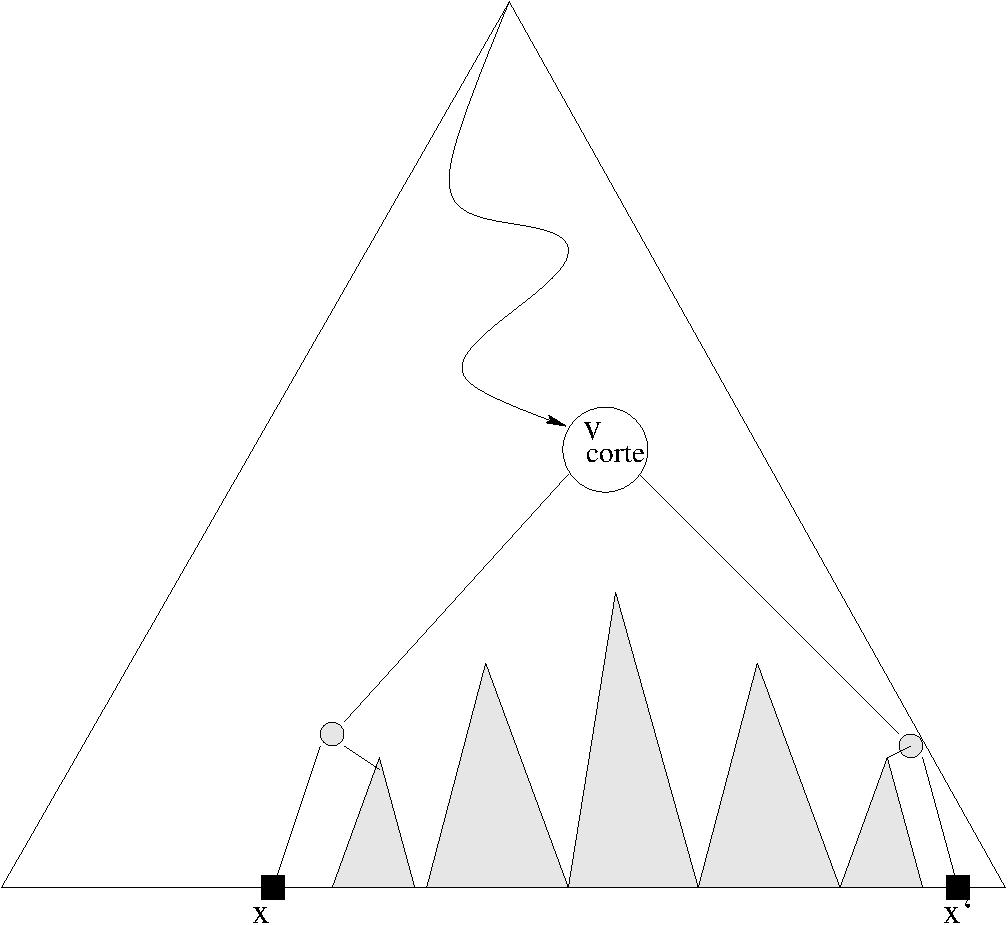
\includegraphics[scale=0.4]{images/range_tree2.pdf}
    \end{center}
    \caption{Consulta de alcance unidimensional, e o $nó_{corte}$ sendo o primeiro nó da consulta}
\end{figure}


Dado o intervalo da consulta $R = [x , x']$ e a raiz de $\Gamma$ realizaremos o seguinte algoritmo:
Inicialmente precisamos encontrar o primeiro nó que está contido na consulta. Chamaremos este nó de $nó_{corte}$.
Para encontrar o $nó_{corte}$ faremos uma consulta simples que a partir da raiz $v$ checaremos se $v$
está dentro do intervalo buscado. Se estiver será nosso $no_{corte}$. Do contrario checaremos se $v > x'$
caso seja, $v$ é maior que o maior valor da consulta, então faremos recursivamente a busca por $no_{corte}$
passando o $nó_{esquerda}$ de $v$. Caso $v \leq x$ realizaremos a consulta por $nó_{corte}$ recursivamente
em $no_{direita}$ de $v$.


Munidos de $nó_{corte}$, faremos a consulta para retornar todos os pontos contidos dentro de $R$ na árvore
$\Gamma$.
A partir de $nó_{corte}$, queremos recursivamente buscar os pontos que são menores que $nó_{corte}$ porem
ainda dentro da consulta, e similarmente, os pontos maiores que $nó_{corte}$ ainda dentro do intervalo.
Assim como buscar os pontos maiores que $nó_{corte}$ e dentro da consulta. \cite{cg_search1}

Para buscarmos os valores menores que $nó_{corte}$ iremos realizar uma consulta em profundidade considerando
os nós não folha à esquerda a partir de $nó_{corte}$ checando se valor do nó $v$ é $v > x$. 
Quando essa condição não for mais atendida, ou seja, $nó \leq x$  isso significa que já não mais está
dentro da consulta. Neste ponto checaremos se o nó à direita está dentro da consulta. Caso esteja reportamos.
Durante a busca em profundidade todos os pontos que atendem $v > x$, reportamos a subárvore à direita
deste nó, ou seja, temos certeza que os valores desta subárvore está dentro do intervalo consultado.


A mesma busca em profundidade será realizada para os valores maiores que $nó_{corte}$, checando se 
o $nó < x'$ e reportando todas as subárvores à esquerda que atendem essa condição. E no caso onde essa
condição seja quebrada checando o nó à esquerda e reportando caso dentro do intervalo.

A condição de parada dessa busca em profundidade é caso seja um nó folha, e caso seja, deve se checar
se está dentro do intervalo, caso esteja reporta-o.

Em seguida temos o pseudocódigo para buscar o $nó_{corte}$ e para consulta unidimensional.

\begin{algorithm}[h!]
    \caption{Recebe como parâmetro um nó e uma janela. Devolve o primeiro ponto dentro janela de consulta.}
    \begin{algorithmic}[1]
    \Function{EncontraNóCorte}{$v$, $R:[x, x']$}
        \While{$v$ não é folha}
        \If{$v \in R$ } 
            \Return $v$
        \Else
            \If{$v > R$ }
                \State $v \leftarrow v_{esquerda}$ 
            \Else
                \State $v \leftarrow v_{direita}$
            \EndIf
        \EndIf
        \EndWhile
    \EndFunction
    \end{algorithmic}
\end{algorithm}


\begin{algorithm}[h!]
    \caption{Recebe um nó e uma consulta. Devolve todos os pontos dentro da consulta.}
    \begin{algorithmic}[1]
    \Function{Busca1DEmAlcance}{$v_{corte}$, $R:[x, x']$}
        \If{$v_{corte}$ é folha}
            \If{$v_{corte} \in R$}
                \State Reporta ponto $v_{corte}$
            \EndIf
        \Else
            \State $v \leftarrow filho_{esq}(v_{corte})$
            \While{$v$ não for folha}
                \If{$v > R$}
                    \State \Call{ReportaSubárvore}{$v$}
                    \State $v \leftarrow filho_{esq}(v)$
                \Else
                    \State $v \leftarrow filho_{dir}(v)$
                \EndIf
            \EndWhile
            \If{$v$ é ponto e $v \in R$}
                \State Reporta ponto $v$
            \EndIf
            \State Similarmente, agora segue o caminho $filho_{dir}(v_{corte})$
        \EndIf
    \EndFunction
    \end{algorithmic}
\end{algorithm}
\clearpage


Na \ref{fig:11} temos a árvore construída em relação a coordenada $y$.
Iremos fazer uma consulta unidimensional de intervalo nesta árvore inicialmente.
Seja o intervalo de consulta $R = [-8, 3]$ segue na figura em seguida:

\begin{figure}[h!]
\centering
    \caption {Em azul, a consulta unidimensional em $y$ nos pontos em $P$}
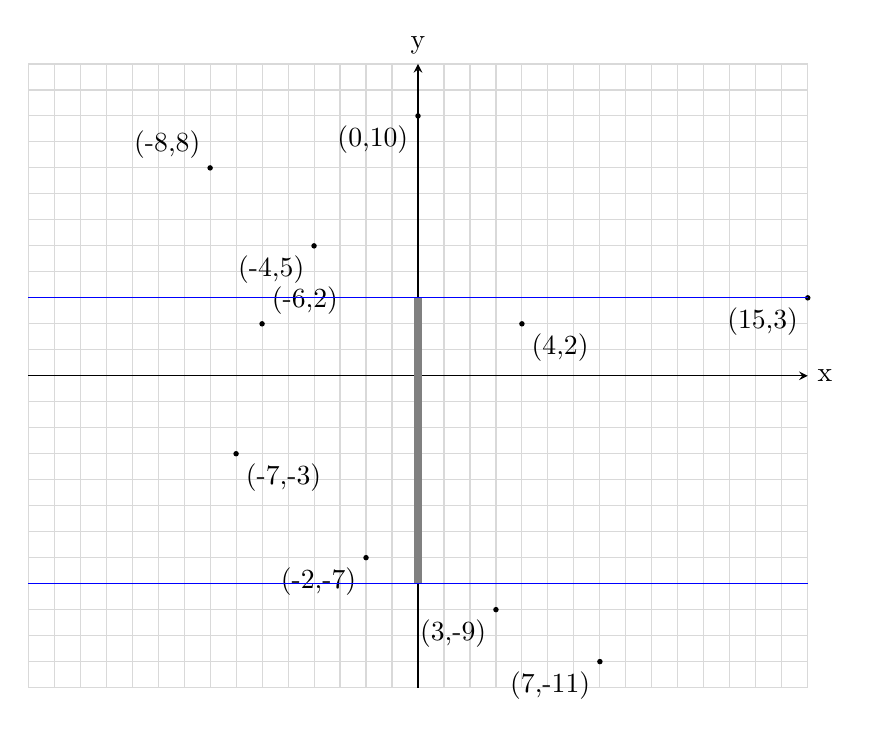
\begin{tikzpicture}[scale=0.33]
  \draw[gray!30] (-15,-12) grid[xstep=1, ystep=1]  (15,12);
  \draw[-stealth] (-15,0)--(15,0) node[right]{x}; % x axis
  \draw[-stealth] (0,-12)--(0,12) node[above]{y}; % y axis


 \fill (15,3)  circle[radius=3pt] node[anchor=north east]{(15,3)};
  \fill (-4,5)  circle[radius=3pt] node[anchor=north east]{(-4,5)};
  \fill (-6,2)  circle[radius=3pt] node[anchor=south west]{(-6,2)};
  \fill (-2,-7)  circle[radius=3pt] node[anchor=north east]{(-2,-7)};
  \fill (3,-9)  circle[radius=3pt] node[anchor=north east]{(3,-9)};
  \fill (0,10)  circle[radius=3pt] node[anchor=north east]{(0,10)};
  \fill (7,-11)  circle[radius=3pt] node[anchor=north east]{(7,-11)};
  \fill (-7,-3)  circle[radius=3pt] node[anchor=north west]{(-7,-3)};
  \fill (-8,8)  circle[radius=3pt] node[anchor=south east]{(-8,8)};
  \fill (4,2)  circle[radius=3pt] node[anchor=north west]{(4,2)};
  
  \draw[draw=gray, line width=3pt] (0,3) -- (0,-8);
  \draw[draw=blue] (-15,3) -- (15,3);
  \draw[draw=blue] (-15,-8) -- (15,-8);

\end{tikzpicture}
\end{figure}


Começamos pelo nó raiz com valor $2$. A condição $-8 \leq 2 \leq 3$ é verdadeira. Portanto $nó_{2}$
será nosso $nó_{corte}$.
A partir dele, primeiramente iremos obter os nós $v$ tal que $v \leq 2$. Começamos a busca em profundidade:
o nó a esquerda de $nó_{2}$ é $no_{-3}$. Reportamos a subárvore à direita $nó_{-3}$ = \{$(-6,2)$\}.
O valor $-3$ ainda mantém $-8 \leq -3$, e, portanto, continuamos a busca em profundidade.

Agora temos o $nó_{-7}$. Por sua vez, satisfaz  $-7 \leq -8$, reportamos a subárvore à direita =\{$(-7, -3)$\}.
A busca em profundidade continuará até o $nó_{raiz}=\{(-2,-7)\}$, que satisfaz a consulta.
Realizaremos o mesmo procedimento, porem, á partir de $nó_{corte}$ iremos realizar busca em profundidade pela direita considerando se o valor do nó é $nó \leq 3$.

Por fim teremos os pontos: \{$(-2,-7), (-7,-3), (-6,2)$\}
\begin{figure}[h]
\centering
\resizebox{.6\textwidth}{!}{
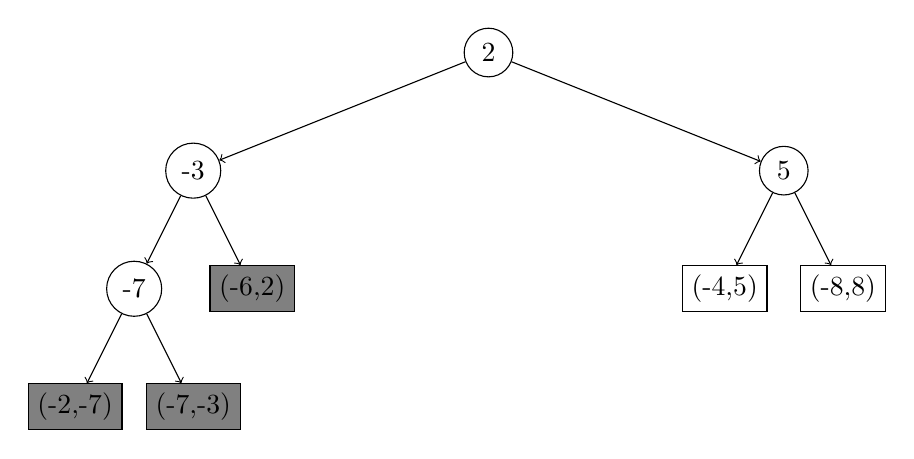
\begin{tikzpicture}[nodes={draw, circle}, ->]
 \node{2}
    child { node {-3} 
        child{ node{-7}
            child{ node[rectangle, fill=gray]{(-2,-7)}}
            child{ node[rectangle, fill=gray]{(-7,-3)}}
        }
        child{ node[rectangle, fill=gray]{(-6,2)}}
    }
    child [missing]
    child [missing]
    child [missing]
    child [missing]
    child { node {5}
        child{ node[rectangle]{(-4,5)}}
        child{ node[rectangle]{(-8,8)}}
    };
\end{tikzpicture}
}
\caption{Pontos na $y$-árvore do $nó_{-6}$}
\end{figure}

\subsection{Consulta Bidimensional}

Para realizar uma consulta bidimensional, iremos realizar uma consulta de intervalos unidimensional para
cada dimensão. 
Iremos para cada nó visitado que está dentro da janela de consulta, será feita outra busca unidimensional
na árvore $\tau$ associada ao nó.
Segue pseudocódigo pra consulta bidimensional:

\begin{algorithm}[h!]
    \caption{Recebe um nó e uma consulta. Devolve todos os pontos dentro da consulta.}
    \begin{algorithmic}[1]
    \Function{Busca2DEmAlcance}{$v_{corte}$, $R : [x,x'] \times [y,y']$}
        \State $v_{corte} \leftarrow$ \Call{EncontraNóCorte}{$\tau$, $x, x'$}
        \If{$v_{corte}$ é folha}
            \State Checa se o ponto em $v_{corte}$ deve ser reportado
        \Else
            \State $v \leftarrow $ $filho_{esq}(v_{corte})$
            \While{$v$ não é folha}
                \If{$x \leq v$}
                    \State \Call{Busca1DEmAlcance}{$filho_{dir}(v) \rightarrow \tau_{associada}, y,y'$}
                    \State $v \leftarrow filho_{esq}(v)$
                \Else
                    \State $v \leftarrow filho_{dir}(v)$
                \EndIf
            \EndWhile
            \State Checa se o ponto está dentro da consulta
            \State Similarmente, agora segue o caminho $filho_{dir}(v_{corte})$
            \State Chamar \Call{Busca1DEmAlcance}{$v \rightarrow \tau_{associada}, y,y'$} nas subárvores associadas
            \State E checar se o ponto associado aos nós folhas tem de ser reportados
        \EndIf
    \EndFunction
    \end{algorithmic}
\end{algorithm}
\clearpage


Iremos agora demonstrar uma consulta bidimensional:
Seja o intervalo de consulta $R = [-6, 1] \times [-8, 3]$
Como explicitado, será uma junção de consultas unidimensionais na $x$-árvore com a consulta $[-6,1]$ e uma consulta nas $y$-árvores associadas entre $[3,-8]$

\begin{figure}[h]

    \centering
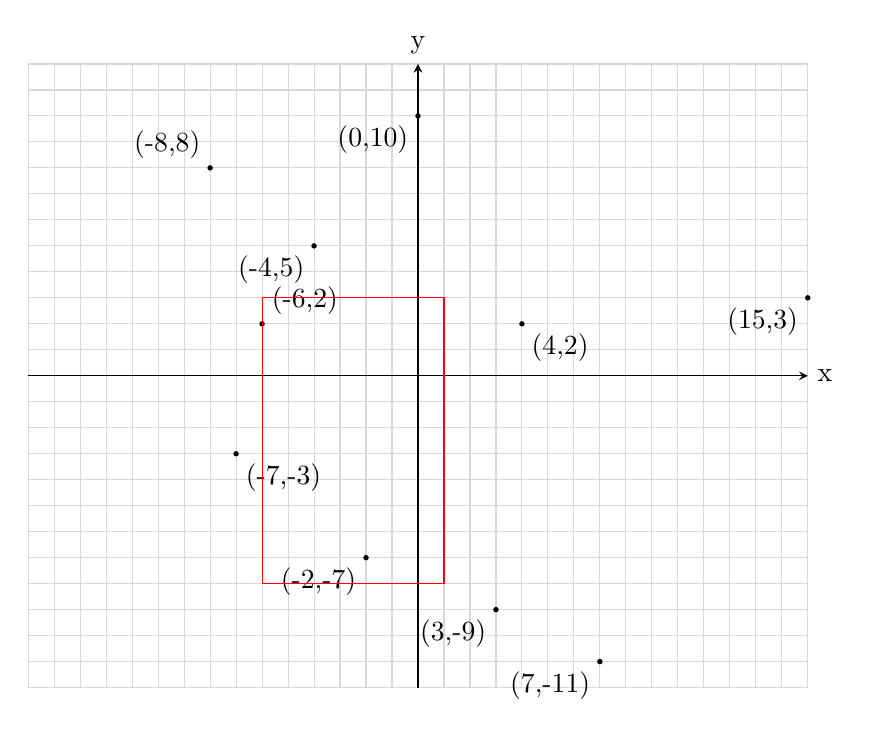
\begin{tikzpicture}[scale=0.33]
  \draw[gray!30] (-15,-12) grid[xstep=1, ystep=1]  (15,12);
  \draw[-stealth] (-15,0)--(15,0) node[right]{x}; % x axis
  \draw[-stealth] (0,-12)--(0,12) node[above]{y}; % y axis


 \fill (15,3)  circle[radius=3pt] node[anchor=north east]{(15,3)};
  \fill (-4,5)  circle[radius=3pt] node[anchor=north east]{(-4,5)};
  \fill (-6,2)  circle[radius=3pt] node[anchor=south west]{(-6,2)};
  \fill (-2,-7)  circle[radius=3pt] node[anchor=north east]{(-2,-7)};
  \fill (3,-9)  circle[radius=3pt] node[anchor=north east]{(3,-9)};
  \fill (0,10)  circle[radius=3pt] node[anchor=north east]{(0,10)};
  \fill (7,-11)  circle[radius=3pt] node[anchor=north east]{(7,-11)};
  \fill (-7,-3)  circle[radius=3pt] node[anchor=north west]{(-7,-3)};
  \fill (-8,8)  circle[radius=3pt] node[anchor=south east]{(-8,8)};
  \fill (4,2)  circle[radius=3pt] node[anchor=north west]{(4,2)};
  
  \draw[draw=red] (-6,3) rectangle (1,-8);

\end{tikzpicture}
\caption {Em vermelho a região do retângulo de consulta}
\end{figure}

Iniciamos a busca no nó raiz $nó_{-2}$. Temos que inicialmente encontrar o $nó_{corte}$ e $nó_{-2}$ está dentro de $[-6, 1]$. 

% Então para encontrarmos $nó_{corte}$ iremos \Call{EncontraNóCorte}{$nó_{2}$,$[-8,-2]$}. 
% $v_{2}$ não é folha, porem não está dentro do intervalo $[-8,-2]$, checamos se $v_{2} > [-8, -2]$, o que é verdadeiro, então iremos checar se o $nó_{-6}$ está dentro do intervalo. Retornamos o $nó_{-6}$ como $nó_{corte}$.

A partir dele faremos uma busca em profundidade para esquerda e para a direita para encontrar todos 
os valores dentro do intervalo $[-6,1]$. 

Como na Figura 8, agora estamos no $nó_{-2}$, este não é folha, então prosseguimos.
Consultaremos em profundidade iniciando pela esquerda. À esquerda de $nó_{-2}$ é $nó_{-6}$, não folha, e portanto checaremos se este está ainda é menor que a consulta, ou seja, se a busca em profundidade pode prosseguir consultando os ramos à esquerda da árvore. $-6 \leq -6$, logo, faremos uma \Call{Busca1DEmAlcance}{$nó_{-4}\rightarrow \tau_{assoc}, -8, 3$}. A árvore auxiliar do $nó_{-4}$ é $\tau_{assoc}$ é a árvore que segue:


\begin{figure}[h]
    \centering
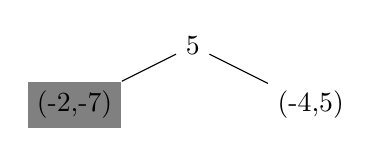
\begin{tikzpicture}[scale=0.5][nodes={draw, circle}, ->]
 \node{5}
    child{ node[rectangle,  fill=gray]{(-2,-7)} }
    child [missing]
    child [missing]
    child [missing]
    child{ node[rectangle]{(-4,5)}};
\end{tikzpicture}
\caption{Pontos na $y$-árvore do $nó_{-4}$}
\end{figure}

Consultaremos nesta árvore os pontos dentro do intervalo $[-8, 3]$, que retornará os pontos em cinza = \{$(-2,-7)$\}.
Consultaremos o próximo nó à esquerda, $nó_{-7}$. Por sua vez a consulta $-6 \leq -7$ é falso e iremos avaliar o nó à direita de $nó_{-7}$ que é o ponto $(-6, 2)$ e checamos se está na janela e o retornamos.
Prosseguiremos com a consulta à direita do $nó_{corte}= nó_{-2}$.

A figura a seguir é a nossa implementação da Árvore de alcance 2D:

\begin{figure}[h]
\centering
\begin{minipage}{.5\textwidth}
  \centering
  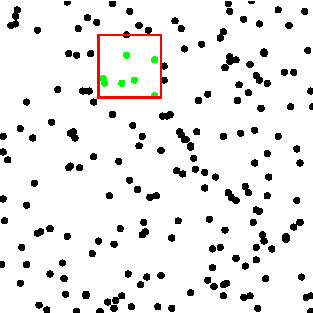
\includegraphics[width=.8\linewidth]{images/rt_t1.pdf}

  \label{fig:test1}
\end{minipage}%
\begin{minipage}{.5\textwidth}
  \centering
  
  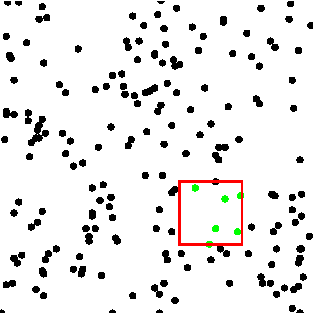
\includegraphics[width=.8\linewidth]{images/rt_t2.pdf}
  \label{fig:test2}
 
\end{minipage}
 \caption{Resultados das consultas em janela com Árvore de Alcance 2D}
\end{figure}

% ----------------------------------------------------------